\RequirePackage[l2tabu,orthodox]{nag}

% TODO: decide if one-sided/two-sided
%\documentclass[headsepline,footsepline,footinclude=false,fontsize=11pt,paper=a4,listof=totoc,bibliography=totoc,BCOR=12mm,DIV=12]{scrbook} % two-sided
\documentclass[headsepline,footsepline,footinclude=false,oneside,fontsize=11pt,paper=a4,listof=totoc,bibliography=totoc]{scrbook} % one-sided

\PassOptionsToPackage{table,svgnames,dvipsnames}{xcolor}

\usepackage[utf8]{inputenc}
\usepackage[T1]{fontenc}
\usepackage[sc]{mathpazo}
\usepackage[american]{babel}
\usepackage[autostyle]{csquotes}
\usepackage[%
  backend=bibtex,
  url=false,
  style=alphabetic,
  maxnames=4,
  minnames=3,
  maxbibnames=99,
  firstinits,
  uniquename=init]{biblatex} % TODO: adapt bibliography style
\usepackage{graphicx}
\usepackage{scrhack} % necessary for listings package
\usepackage{listings}
\usepackage{lstautogobble}
\usepackage{tikz}
\usepackage{pgfplots}
\usepackage{pgfplotstable}
\usepackage{booktabs}
\usepackage[final]{microtype}
\usepackage{caption}
\usepackage[hidelinks]{hyperref} % hidelinks removes colored boxes around references and links
\usepackage[toc,nonumberlist,acronym]{glossaries} % TODO: remove if glossary not needed
\usepackage{amsmath}
\usepackage{epstopdf}
\usepackage{psfrag}
\usepackage{longtable}
\bibliography{references/literature}

\setkomafont{disposition}{\normalfont\bfseries} % use serif font for headings
\linespread{1.05} % adjust line spread for mathpazo font

% Settings for glossaries TODO: remove the following block if glossary not needed
\renewcommand{\glsnamefont}[1]{\normalfont\bfseries #1} % use serif font for glossary entry titles
\makeglossaries{}

% Settings for pgfplots
\pgfplotsset{compat=1.9} % TODO: adjust to your installed version
\pgfplotsset{
  % For available color names, see http://www.latextemplates.com/svgnames-colors
  cycle list={CornflowerBlue\\Dandelion\\ForestGreen\\BrickRed\\},
}

% Settings for lstlistings
\lstset{%
  basicstyle=\ttfamily,
  columns=fullflexible,
  autogobble,
  keywordstyle=\bfseries\color{MediumBlue},
  stringstyle=\color{DarkGreen}
}

% Basic information for cover & title page
\newcommand*{\getUniversity}{Technische Universität München}
\newcommand*{\getFaculty}{Department of Informatics}
\newcommand*{\getTitle}{Control of Modular Robots}
%\newcommand*{\getTitleGer}{}
\newcommand*{\getAuthor}{Authors}
\newcommand*{\getDoctype}{Report for Practical Course}
\newcommand*{\getSupervisor}{Supervisor}
%\newcommand*{\getAdvisor}{Prof. Dr.-Ing. Matthias Althoff}
\newcommand*{\getSubmissionDate}{02.07.2015}
\newcommand*{\getSubmissionLocation}{Munich}

% TODO: add custom commands etc.


% TODO: remove if glossary not needed
% \newglossaryentry{V(t)}
{
  name=V(t),
  description={is the appled voltage}
}
\newglossaryentry{L}
{
  name=L,
  description={is the armature self inductance}
}
\newglossaryentry{R}
{
  name=R,
  description={is the armature resistene}
}
\newglossaryentry{\(V_{b}\)}
{
  name=\(V_{b}\),
  description={is the back emf constant}
}
\newglossaryentry{\(\theta_{m}\)}
{
  name=\(\theta_{m}\),
  description={is the mechanical rotor angle}
}
\newglossaryentry{\(\tau_{m}\)}
{
  name=\(\tau_{m}\),
  description={is the generated torque}
}
\newglossaryentry{\(\tau_{l}\)}
{
  name=\(\tau_{l}\),
  description={is the load torque}
}
\newglossaryentry{i(t)}
{
  name=i(t),
  description={is the induced current}
}

\newglossaryentry{
\(V_{L}\) }
{
  name=
i(t) ,
  description={is the inductance times the first derivative of the induced current}
}
\newglossaryentry{\(V_{R}\)}
{
  name=\(V_{R}\),
  description={is the resistence times the induced current}
}
\newglossaryentry{\(V_{emf}\)}
{
  name=\(V_{emf}\),
  description={is the back induced electromotive force}
}
\newglossaryentry{\omega(t)}
{
  name= \omega(t),
  description={is the angular velocity seen at the shaft}
}
\newglossaryentry{\(\(K_m\)}
{
  name=\(\(K_m\),
  description={is the torque constant}
}
\newglossaryentry{u(t)}
{
  name=u(t),
  description={is the torque seen at the shaft}
}
\newglossaryentry{Z}
{
  name=Z,
  description={rotation around Z-axis}
}
%\newacronym{tum}{TUM}{Technische Universität München}
\newacronym{V(t){}{Applied voltage}
\newacronym{L}{Armature self inductance}
\newacronym{R}{Armature resistence}
\newacronym{\(V_{b}\)}{Back emf constant}
\newacronym{\(\theta_{m}\)}{Mechanical rotor angle}
\newacronym{\(\tau_{m}\)}{Generated torque}
\newacronym{\(\tau_{l}\)}{Load torque}
\newacronym{i(t)}{Induced current}
\newacronym\(V_{L}\){Inductance times derivative of induced current}
\newacronym{\(V_{R}\)}{Resistence times induced current}
\newacronym{\(V_{emf}\)}{Back induced electromotive force}
\newacronym{ \omega(t)}{Angular velocity seen at shaft}
\newacronym{\(\(K_m\)}{Torque constant}
\newacronym{u(t)}{Torque seen at the shaft}
\newacronym{Z}{Rotation around Z-axis}


\begin{document}

%\input{pages/cover}

\frontmatter{}

\begin{titlepage}
  \centering

  \vspace{40mm}
  
\includegraphics[width=40mm]{logos/tum}

  \vspace{5mm}
  {\huge\MakeUppercase{\getFaculty{}}}\\

  \vspace{5mm}
  {\large\MakeUppercase{\getUniversity{}}}\\

  \vspace{20mm}
  {\Large \getDoctype{}}

  \vspace{15mm}
  {\huge\bfseries \getTitle{}}

  \vspace{10mm}
 % {\huge\bfseries \getTitleGer{}}

  \vspace{15mm}
  \begin{tabular}{l l}
    Authors: & \getAuthor{} \\
    Supervisor: & \getSupervisor{} \\
    %Advisor: & \getAdvisor{} \\
    Submission Date: & \getSubmissionDate{} \\
  \end{tabular}

  \vspace{20mm}
  %
\includegraphics[width=20mm]{logos/faculty}
\end{titlepage}

%\input{pages/disclaimer}
%\input{pages/acknowledgements}
\chapter{\abstractname}


In this course our team implements the dynamic model of Schunk`s  reconfigurable modular robot manipulator LWA 4P. We use Matlab and Simulink to implement the single modules. For that we first obtain the Equations of Motion using the Newton-Euler-formulation. We characterize the modules for an automatic modelling method by providing estimates for masses and inertia tensors using measurements and CAD data, so that the EoM can be automatically achieved. We then provide the preliminary Simulink model for the robotic arm.  Secondly, we identify the dynamic modell of the actuators. With Black-Box identification and with White-Box identification. In the next step, we implement a simulator of the robot by enhancing the simulink model including saturation effects and possible delays and validate the model using measurements. The fourth step is to design and tune the decentralized controllers while considering limitations due to the sampling time and test them on the robot. We finally test the controllers with a trajectory planner modelling the kinematic behaviour, which is developed by our second team.


\microtypesetup{protrusion=false}
\tableofcontents{}
\microtypesetup{protrusion=true}
\microtypesetup{protrusion=true}


\mainmatter{}

\chapter{Introduction}\label{chapter:introduction}

As robots are getting more and more complicated, modular robots play an important role in robotics. Modular robots consist of independent cubes, which can connect themselves in different ways in order to fulfill a task. Each of the cubes has its own power supply and intelligence and can have specific tools for solving a problem under special conditions. After a computer has been fed a problem, it analyzes it and connects to the cubes in such a way that it can solve the problem. The cubes have the same size in modular robots in opposite to fractal robots, which can have cubes of different sizes. The cubes can be practically identical built, with similar software implementations, so that the input data and combinations of moduls determines how the task is executed.
\chapter{Obtaining the Equations of Motion using the Newton-Euler formulation and 
creating a preliminary Simulink model of the robotic arm}\label{chapter:1}
\vspace{-0.25cm}
Responsible: \textit{Sophie Sepp and Benedict Feldotto}

\section{Obtaining the Equations of Motion using the Newton-Euler formulation}
In chapter two a preliminary Simulink model of the robotic arm is created using the Newton Euler Formulation of the Equations of Motion. 



\subsection{Theoretical background}
To derive the equations of motion of the manipulator we use the Newton Euler Method. The equations of motion are used to compute the dynamic model of the robot. While in the Euler-Lagrange Equations the manipulator is treated as a whole and the analysis is performed using a Lagrangian function, in the Newton-Euler formulation each link of the robot is treated in turn.  Since each link is coupled to other links, the forces and torques of a link also appear in the equations describing its neighboring links. The whole process of deriving the terms of each link is called a forward-backward recursion.
In the forward phase we obtain the rotational velocities and accelerations using the following equations, where i+1 denotes the following link to the link i.


\begin{figure}[htsb]
  \centering
  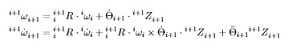
\includegraphics{figures/Rotational velocities and accelerations.jpg}
  \caption{Rotational velocities and accelerations.}
\end{figure}

\\For the linear accelerations of the single joints we use the formula:
\ \\
\begin{figure}
  \centering
  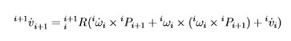
\includegraphics{figures/Linear accelerations of single joints.jpg}
  \caption{Linear accelerations of single joints.}
\end{figure}





\\To find the linear acceleration of the center of mass of each link we use:







\ \\
\begin{figure}[htsb]
  \centering
  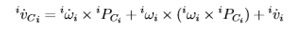
\includegraphics{figures/Linear acceleration for the center of mass of each link.jpg}
  \caption{Linear acceleration for the center of mass of each link.}
\end{figure}







\\In the backwards phase we use the following equations to compute the forces and torques at the center of mass of each link und the forces and torques acting on each joint:




\begin{figure}[htsb]
  \centering
  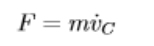
\includegraphics{figures/Equation Force.jpg}
  \caption{Equation Force.}
 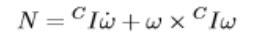
\includegraphics{figures/Equation Torque 1.jpg}
  \caption{Equation Torque 1.}
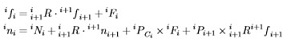
\includegraphics{figures/Forces and torques acting on each joint.jpg}
  \caption{Forces and torques acting on each joint.}
\end{figure}


  





\subsection{Implementing the equations in Matlab}
We first create a Simulink model of three links connected to the given initial constants and to the end effector. Each matlab function block holds a function to compute with the given input parameters the output parameters which become the input parameters of the next link. Thus all links are connected and compute the next values according to the input values they get from the previous link. This is done for the forward phase as well as for the backward phase. In the forward phase the linear and rotational velocities and accelerations of each link are computed. In the backwards phase the forces and torques that act on the centers of mass of each link are computed (Fi, Ni) and the forces and the torques that act on the single joints (fi, ni).



\begin{figure}[htsb]
  \centering
  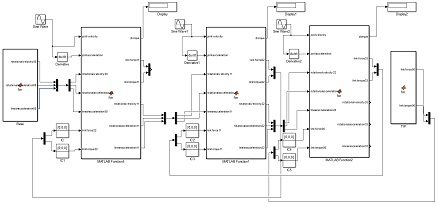
\includegraphics{figures/Three Links.jpg}
  \caption{Three Links.}
\end{figure}

\clearpage
\section{Implementing the Simulink Model}



\chapter{Deriving a dynamical model of the actuators and combining it with the Simulink Model of chapter 2.2}\label{chapter:2}
\vspace{-0.25cm}
Responsible: \textit{Sophie Sepp}


\ \\

In task 2 a dynamical model of the actuators is derived and the Simulink model of task 1.ii is enhanced with the actuator models. The robotic arm LWA 4P has six brushless DC motors which are modelled in Simulink and combined with the Simulink model of task 1. The modelling of the motor is hereby divided by the electrical part of the motor equations and the dynamical part of the motor equations.

\section{Deriving a dynamical model of the actuators }


\subsection{Theoretical background: DC motor}
A DC-motor works on the principle that a current-carrying conductor in a magnetic field experiences a force, which can be expressed as the product of magnetic flux and the current in the conductor. It consists of a fixed stator, which provides a constant magnetic field and a armature part, which is a rotor that rotates inside the stator and is a simple coil. The armature is connected to a DC power source through a pair of commutator rings. The current that flows through the coil induces a electromagnetic force on it according to the Lorentz force, which causes the coil to rotate. Thus the commutator rings connect with the  power source of opposite polarity. As a result, on the left side electricity flows away while on the right side, electricity flows towards. Thus the torque action is in the same direction throughout the motion, which is the reason why the coil continues rotating. 
A characteristical aspect of DC motors is the production of back emf. A rotating loop in a magnetic field produces an emf according to the principle of electromagnetic induction, which are in this case the armature loops. So an internal emf will be induced, that opposes the applied input voltage. 
\begin{figure}[htsb]
  \centering
  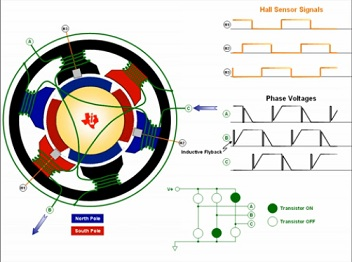
\includegraphics{figures/DC-motor.jpg}
  \caption{DC motor.}
\end{figure}




\clearpage


\subsection{Equations describing DC motor}

 Electrical part of the motor equations:

\begin{figure}[htsb]
  \centering
  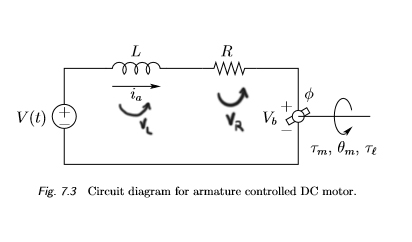
\includegraphics{figures/Circuit diagram for armature controlled DC motor.jpg}
  \caption{Circuit diagram for armature controlled DC motor.}
\end{figure}

V(t): Applied voltage\\
L: Armature self inductance\\
R: Armature resistence\\
\(V_{b}\): Back emf constant\\
\(\theta_{m}\): mechanical rotor angle\\
\(\tau_{m}\): generated torque\\
\(\tau_{l}\): load torque\\




\ \\
The voltage Vl and Vr can be computed in the following way: \\

\(V_{L}\) = \(L \cdot  \(\frac{di}{dt}\) \) \\

\(V_{R}\) = \(R \cdot i \) 



\clearpage

The electrical part of the motor can be computed by the sum of  Vl, Vr and the back emf. \\


\(V_{t}\)(t) = \(L \cdot \frac{di}{dt} \)+\(R \cdot i(t) \) + \(V_{emf}\) \\


The back (induced) electromotive force Vemf is proportional to the angular velocity ω(t) seen at the shaft.  Vb, the emf constant, also depends on certain physical properties of the motor. \\

\(V_{emf}\)(t) = \(\(V_{b}\) \cdot \omega(t) \) \\

The mechanical part of the motor equations is derived using Newton's law:  \\



\(J \cdot \(\frac{d\omega}{dt}\)  \)= \(\sum \limits_{i=1}^n \(\tau_i\)=\(- \(V_b\) \cdot \omega(t) \) + \(\(K_m\) \cdot i(t) \)  \\

The inertial load J times the derivative of angular rate equals the sum of all the torques about the motor shaft and can be expressed by the sum of the induced current i times the torque constant Km and the negative product of the back emf constant Kb and the angular velocity ω.

Moreover, the torque u seen at the shaft of the motor is proportional to the current i and can be expressed as the product of the current i and the torque constant Km, which is related to physical properties of the motor, such as magnetic field strength. \\


u(t) = \(\(K_m\) \cdot i(t) \)





\chapter{Conclusion}\label{chapter:conclusion}

...

\appendix{}

 % TODO: remove if glossary not needed
% \glsaddall{} % add all defined terms to glossary, even if not referenced in text
% \printglossaries{}


\microtypesetup{protrusion=false}
\listoffigures{}
\listoftables{}
\microtypesetup{protrusion=true}

\renewcommand{\bibname}{References}
\printbibliography{}


\end{document}






